\chapter{Kapcsolódó kutatások}
\label{ch:related_research}

\section{Hulladékdetektálási módszerek}
\label{ch:waste-detection-methods}

A hulladékdetektálás témája viszonylag új, és számos fejlemény történt az évek során, tekintve, hogy a légi és műholdfelvételek minősége is nőtt. Emiatt kevés olyan kutatás létezik, mely pontosan azzal a problémával foglalkozik, amivel ebben a dolgozatban foglalkoztam, de az érintőleges kutatások is olyan módszereket, ötleteket mutatnak be, melyeket érdemes megfontolni ebben a kutatásban is. Az én kutatásom a Térinformatikai kutatólabor munkájára épül \cite{magyar2023}, ahol egy Random Forest modell került betanításra, hulladékdetektálás céljából. A kutatásban PlanetScope és Sentinel-2 műholdfelvételeket használtak. Ez a cikk rakta le az alapjait az én kutatásomnak is, melyben ezeken az eredményeken javítok. A cikkben további lehetséges munkaként említésre kerül a modell több adattal való tanítása, illetve a képfeldolgozás gyorsítása. A dolgozatom mindkét feladattal foglalkozik, A dolgozatomban csak a PlanetScope felvételek kerülnek felhasználásra, mivel a magasabb felbontású felvételek könnyebben lehetővé teszik a tanító adatok előállítását, hiszen jobban lehet látni a hulladéklerakókat rajtuk.

\cite{sakti2023}-ben Sentinel-2 műholdfelvételeken tanítottak be egy Random Forest modell-t azzal a céllal, hogy egy indonéziai folyóban detektáljanak hulladékot. A cikkben bevezetik az "Adjusted Plastic Index"-et, mellyel a vegetáció, föld és épületek közötti zajt csökkentik. Ennek az indexnek a kiszámításához a Sentinel-2 műhold piros, közeli infravörös (NIR), illetve rövid hullámhosszú közeli infravörös (SWIR) sávokat használták fel. Validációnak Pleiades műholdképeket és drónfelvételeket klasszifikáltak Mahalanobis távolság gépi tanulási módszerrel (\ref{fig:sakti} ábra). A módszer növényzeten és vízen rendre 88\%, illetve 85\% pontosságot ért el és épületeken, törmeléken és földön rendre 62\%, 53\%, illetve 21\% pontossággal tudta a hulladékot detektálni. A cikk szerint az utóbbi három adattípuson azért visszafogottabbak az arányok, mert a spektrális értékei az épületeknek, a földnek és a törmeléknek nagyon hasonlítanak.

\begin{figure}[H]
	\centering
	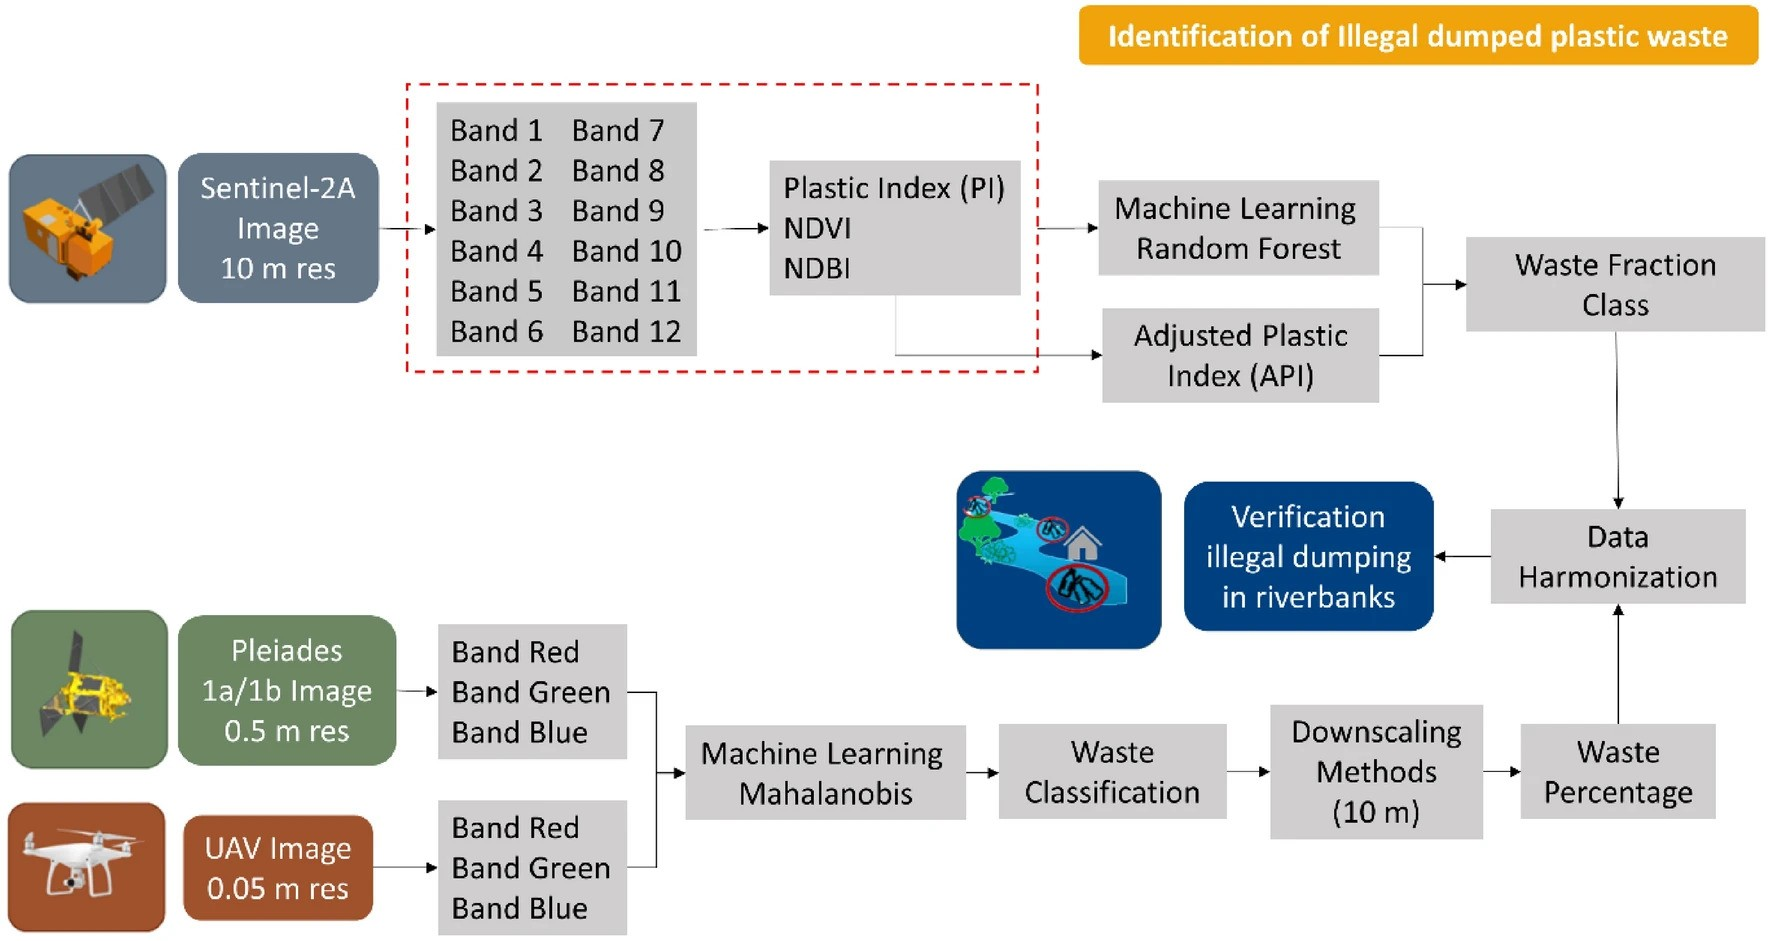
\includegraphics[width=0.6\textwidth,frame]{sakti}
	\caption{Hulladékdetektálás "Adjusted Plastic Index", Random Forest és Mahalanobis távolság segítségével \cite{sakti2023}}
    \label{fig:sakti}
\end{figure}


\cite{goncalves2022}-ben Spectral Angle Mapping módszert alkalmaztak multispektrális drónfelvételeken, egy Portugál tengerparton. A célja a kutatásnak az volt, hogy a tengerparton kimosott hulladékot detektálják és klasszifikálják. A módszer alkalmazásához referencia értékeket állítottak elő azzal, hogy elhelyeztek különböző anyagokból álló hulladékot a homokba, és ezekről drónfelvételt készítettek (\ref{fig:goncalves} ábra). Ezzel a módszerrel képesek voltak detektálni és klasszifikálni nem csak homok fölött található hulladékot, hanem a homokban félig elásott hulladékot is. A 472 kézzel előállított tesztadatból volt a 268 True Positive (57\% összesen), 96 volt a False Positive és 204 volt a False Negative.

\begin{figure}[H]
	\centering
	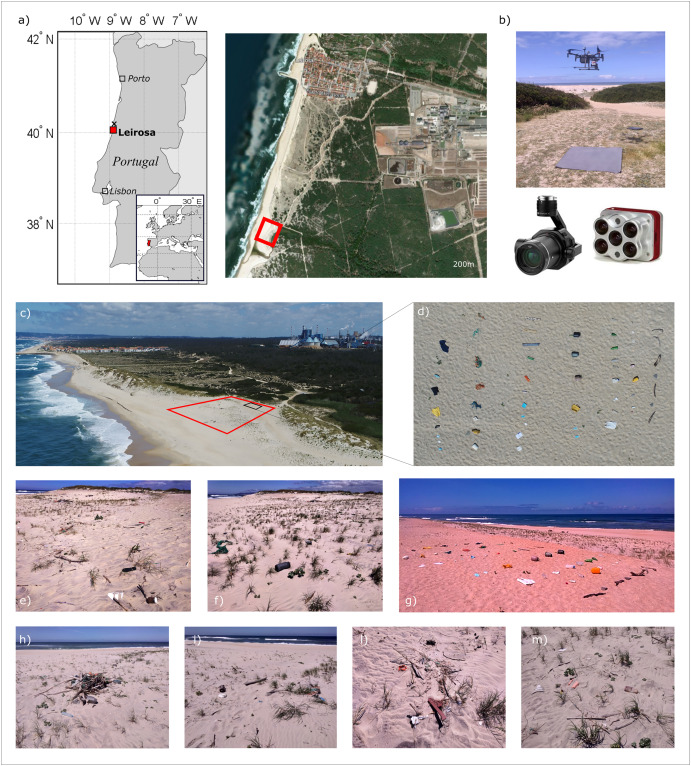
\includegraphics[width=0.6\textwidth,frame]{goncalves}
	\caption{Spectral angle mapping referencia adatainak előállítása \cite{goncalves2022}}
    \label{fig:goncalves}
\end{figure}

\cite{lanorte2017}-ben mezőgazdasági hulladékdetektálásra használtak egy Support Vector Machine modellt, Landsat 8 műholdfelvételeken. A szenzor Kék, Zöld, Piros, NIR, SWIR 1, SWIR 2 és CIRRUS sávját használták a tanító adatok és tesztadatok előállítására. Ezután véletlenszerűen szétválasztották az adatokat tanító adatokra és tesztadatokra. A következő osztályokra bontották az adatokat: Hálók, műanyag takarók, föld, növényzet, gyümölcsöskert, olajfás kert, város, fa, fás föld. A modell a tesztadatokat összességében 94\%-os pontossággal tudta klasszifikálni, ahol a legrosszabb arányokat az olajfás kert érte el 77.78\%-os pontossággal.

\cite{zeng2019}-ben a hiperspektrális adatokon tanítottak be egy felügyelt és egy felügyeletlen gépi tanulási módszert. A működési elv az, hogy a felügyelt módszerrel klasszifikálják a hulladékkal szennyezett területeket, míg a felügyeletlen módszerrel megbecsülik a hulladékkal szennyezett terület kerületét (\ref{fig:zeng} ábra). Ők 99.89\%-os kappa együtthatóval tudtak hulladékot detektálni \todo{Átnézni mégegyszer a cikket és átvizsgálni az adatok helyességét}.

\begin{figure}[H]
	\centering
	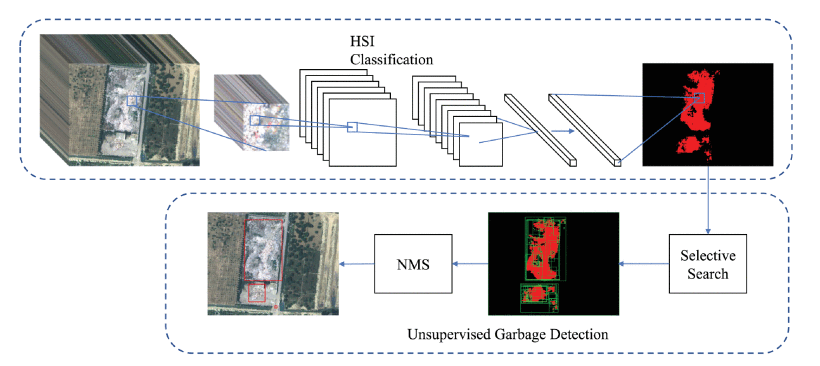
\includegraphics[width=0.6\textwidth,frame]{zeng}
	\caption{Az MSCNN működési elve \cite{zeng2019}}
    \label{fig:zeng}
\end{figure}

\cite{sun2023}-ben megvizsgálják azt, hogy mennyivel lesz hatékonyabb a hulladékkezelés a manuális vizsgálat helyett, ha egy mély tanulás alapú hulladékdetektálási módszert használnak a hulladékkezeléshez magas (0.3m-1m per pixel) felbontású műholdfelvételeken. Négy osztályba bontják a hulladékot: háztartási hulladék, mezőgazdasági hulladék, építkezési hulladék, lefedett hulladék. A modell képes 98\%-át detektálni a hulladéklerakóknak a teszthalmazban, illetve az automata detektálás segítségével több, mint 96.8\%-al csökkentették azt az időt, ami a hulladékdetektálás vizsgálatára kellett. Ráadásul a modell könnyen telepíthető egy laptopra, és 30 másodperc alatt le tudja futtatni a modellt a 162 négyzetkilométeres tesztadathalmazon. A betanításhoz mindössze 2500 hulladéklerakót annotáltak világszerte kézzel 4800 négyzetkilométeren keresztül. A \ref{fig:bca-net-working} ábrából látható a módszer működési elve: a modell a spektrális értékek mellett a hulladéklerakó alakját is figyelembe veszi. A megfelelő magabiztosságú területek hulladéklerakóként lesznek címkézve. A modellt betanító és validáló kód, illetve az adathalmaz, mellyel az eredmények reprodukálhatóak elérhetőek a cikkből.

\begin{figure}[H]
	\centering
	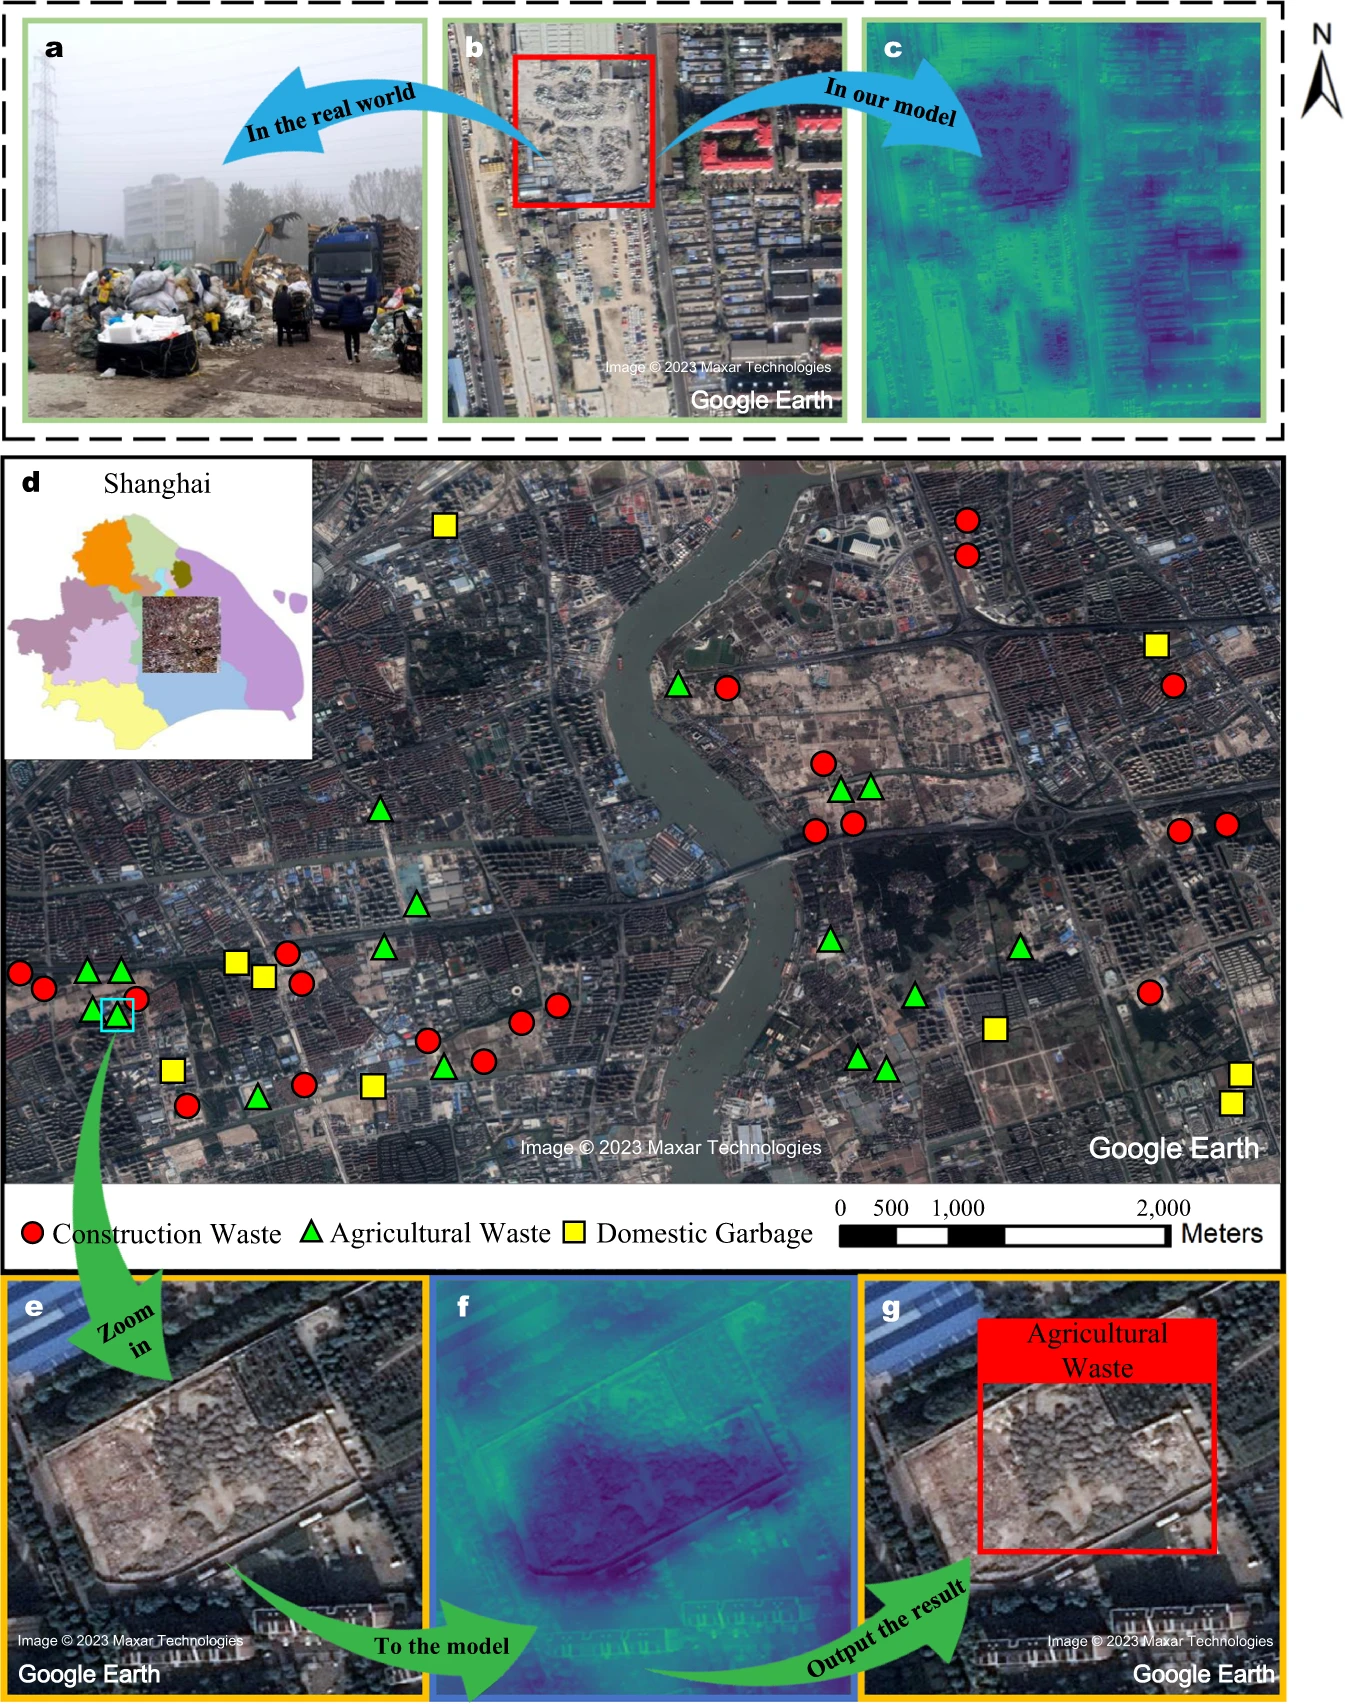
\includegraphics[width=0.6\textwidth,frame]{bca-net}
	\caption{Az BCA-Net működési elve \cite{sun2023}}
    \label{fig:bca-net-working}
\end{figure}

\cite{Torres2021} egy konvolúciós neuronhálót használ, mely 94.5\%-os átlagos pontossággal és 88.2\%-os F-Score-al rendelkezik. A tanító adathalmaz 3000 ortofotóból áll, melyek 20cm per pixel felbontással rendelkeznek és a vörös, kék és zöld tartományokat tartalmazzák. A felvételeket szakértők annotálták, kézzel. A modell a ResNet50 \cite{ResNet2016} hálóra épül és a Feature Pyramid Network \cite{FPN2017} architektúrával van kiegészítve. A modell figyelembe veszi a hulladéklerakó alakját és kontextusát, mely segít a hulladékdetektálás pontosságának a növelésében.

\cite{Page2020}-ban két Random Forest algoritmust tanítottak be kerekek és műanyagok detektálására, Skóciában. A kutatásukban A Copernicus Sentinel-1 és Sentinel-2 multispektrális műholdfelvételeit használták. A tesztelés során a modellek 211 kerék és műanyag alapú hulladéklerakót találtak, rendre 87.5\% és 84\% pontossággal. A kutatásukban az NDVI, SAVI, illetve NDWI2 indexek kerülnek tárgyalásra és kiszámításra.

\cite{Taggio2022} tengeri hulladékdetektálással foglalkozott Görögország területén levő tengerpartokon: egy felügyelt (Light Gradient Boosting Model) és egy felügyeletlen (K-Means) gépi tanulási algoritmust alkalmaztak PRISMA hiperspektrális műholdfelvételeken, mellyel átlagosan 96\%-os pontosságot értek el. A tanító adatokat kontrollált környezetben állították elő (\ref{fig:marine-data-controlled}): különböző környezeteket szimulálva vízre helyeztek különböző anyagokból álló hulladékokat, melyekről műholdfelvételek készültek. Ennek köszönhetően pontosan elő tudták állítani a tanító adatokat \todo{átfogalmazni, mégegyszer elolvasni a cikket}.

\begin{figure}[H]
	\centering
	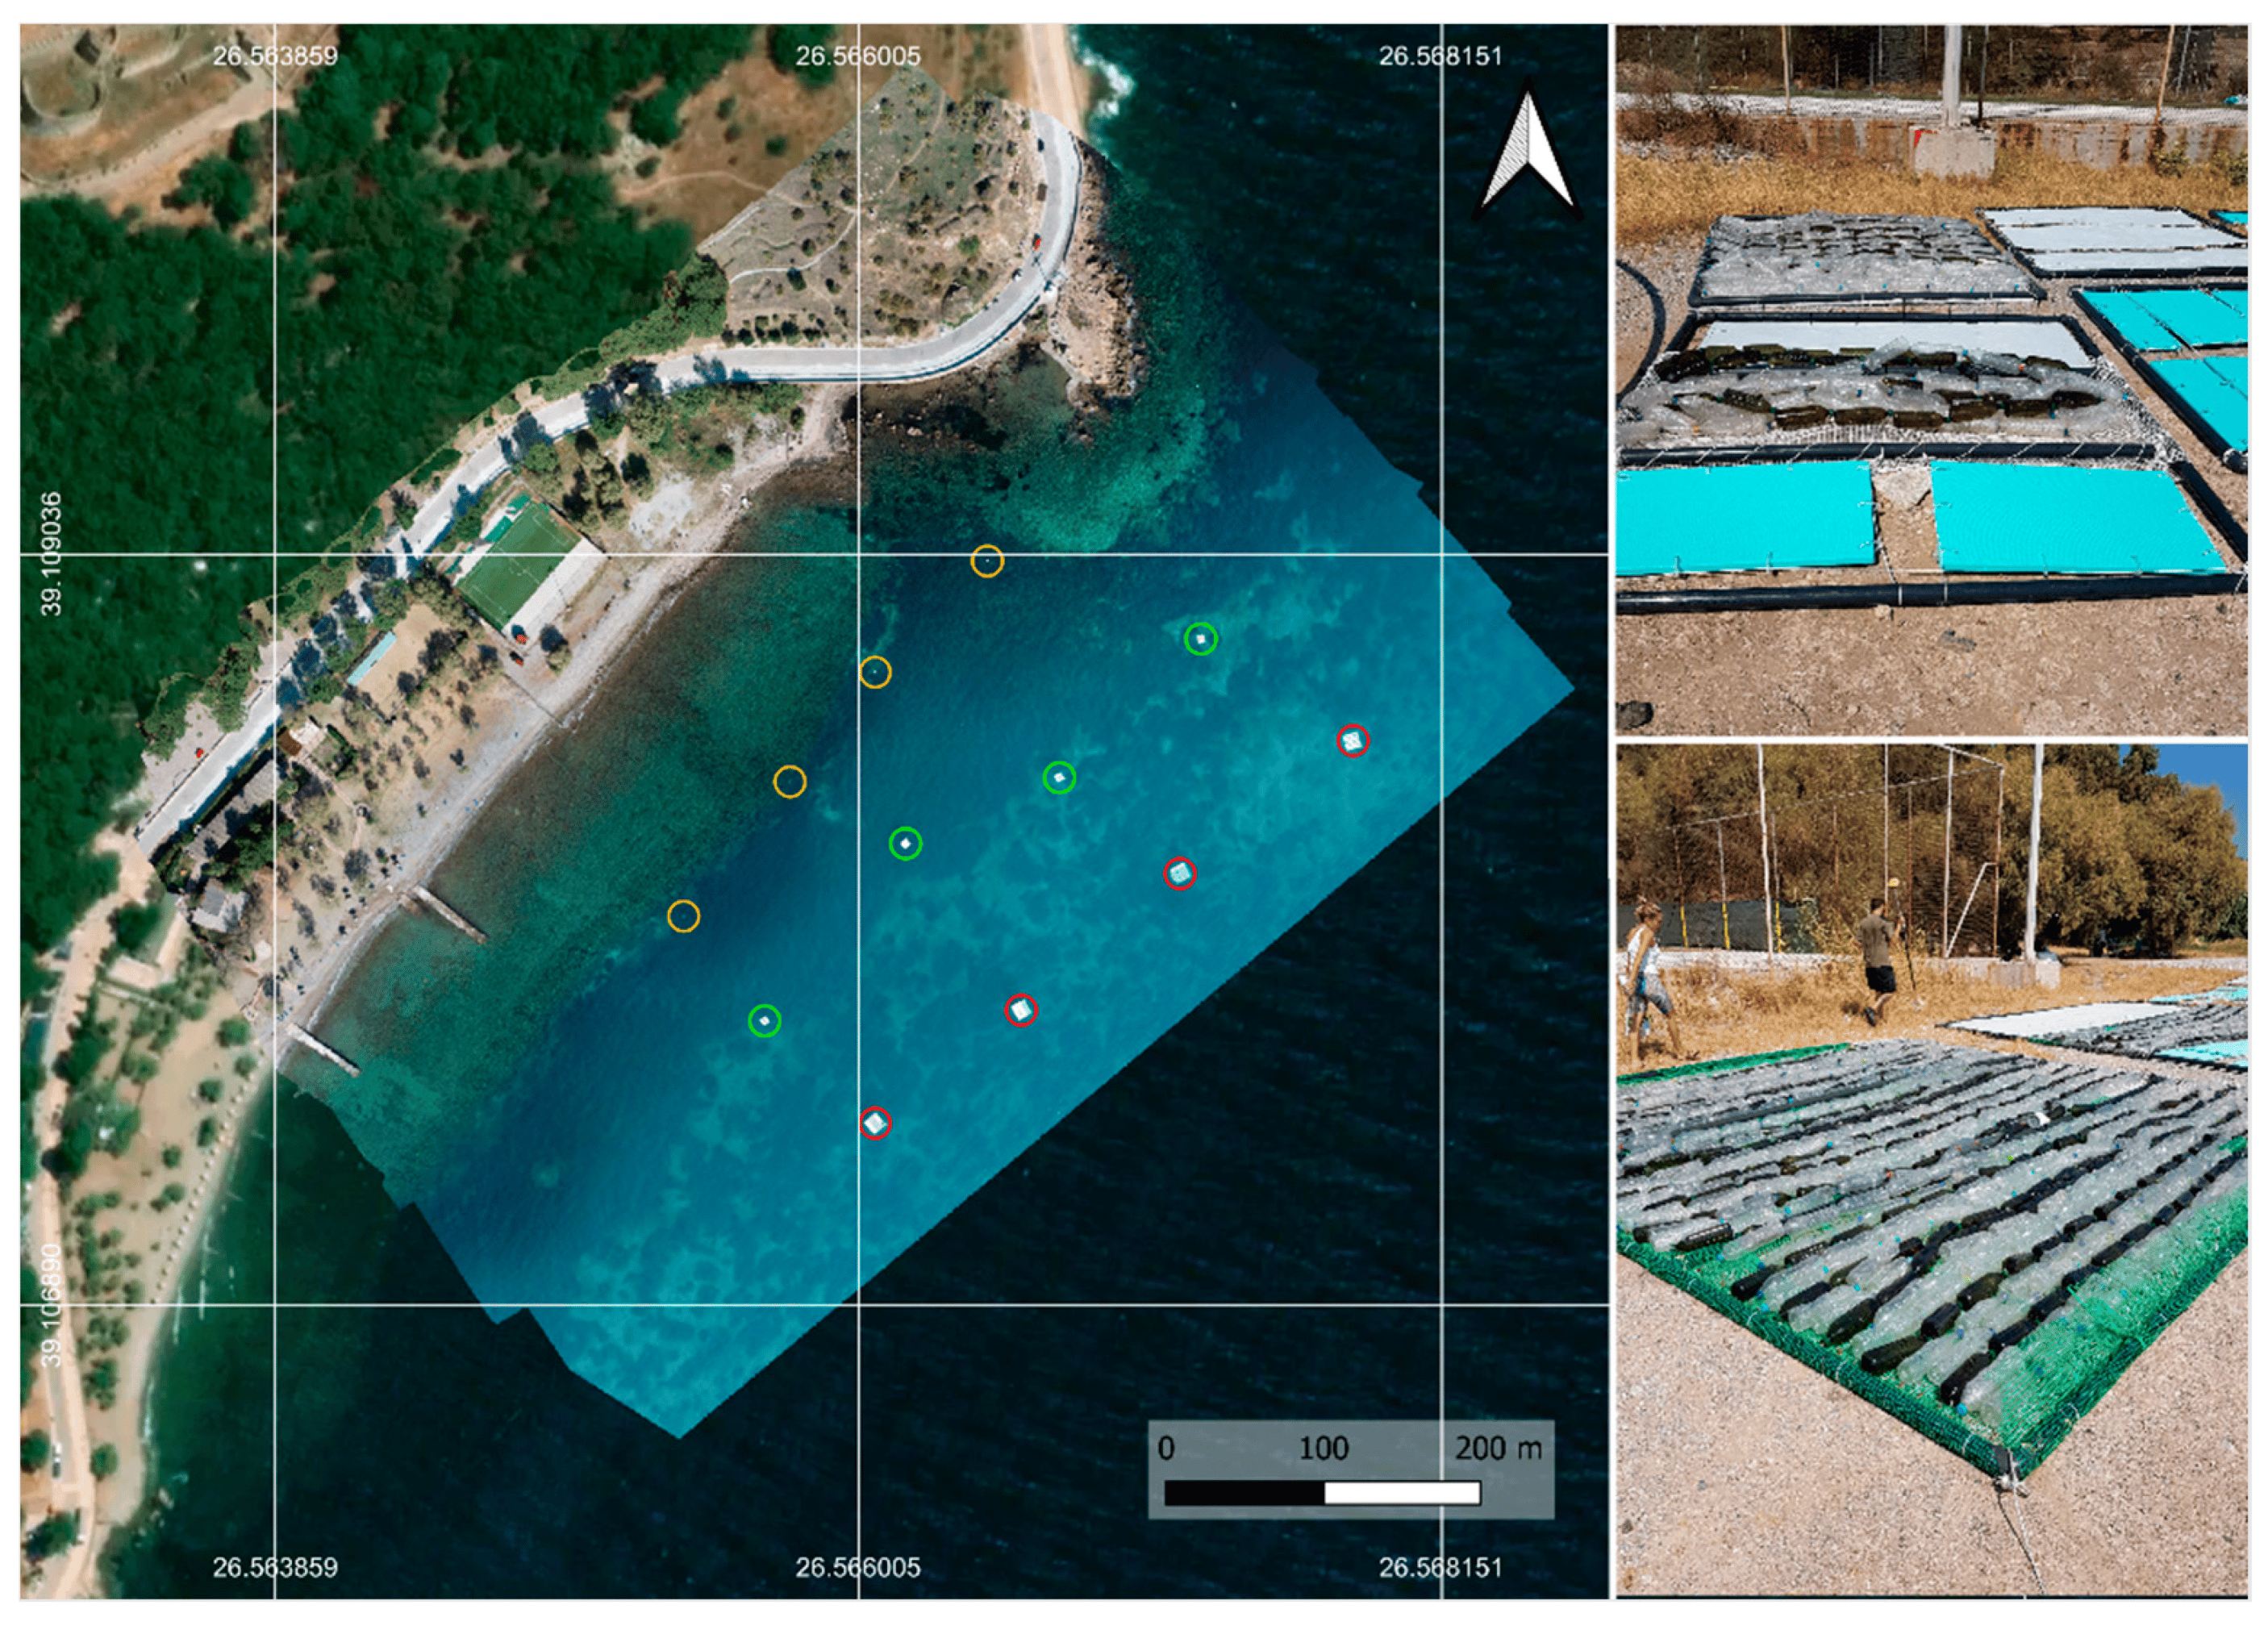
\includegraphics[width=0.6\textwidth,frame]{marine-data-controlled}
	\caption{A tengeri hulladékdetektáláshoz való tanító adatok előállítása \cite{Taggio2022}}
    \label{fig:marine-data-controlled}
\end{figure}

\cite{Wolf2020}-ban tengerparti hulladékdetektálással foglalkoztak, úgy úszó hulladékkal, mint partra kimosott hulladékkal. A kutatásban bemutatnak egy APLASTIC-Q konvolúciós neuronhálót, mely 5 pixel per cm felbontással rendelkező felvételeket klasszifikált Kambodzsa területén . A modell két fő komponensből állt: egy műanyag-hulladék detektálóból (PLD-CNN) és egy műanyag-hulladék osztályozóból (PLQ-CNN). A PLD-CNN megkülönböztette a vizet, homokot, növényzetet és műanyag alapú hulladékot 83\% átlagos pontossággal, illetve megállapította, hogy az adott terület mennyire hulladékos. PLQ-CNN megkülönböztette a különböző hulladék típusokat átlagosan 71\%-os pontossággal: ilyenek például az üvegpalackok, cipők, textil anyagok stb. A PLD-CNN betanításához 5515 darab 100 × 100 × 3 pixeles csempét használtak, míg a PLQ-CNN betanításához 4828 darab 50 × 50 × 3 pixeles csempékre vágták a felvételeket. 

\cite{Goncalves2020}-ban gépi tanulást, geomorfológiát, fotogammetriát és hidrodinamikai modellezést kombinálnak össze azzal a céllal, hogy homokos partok környékén, illetve homokdombokon detektáljanak hulladékot drónfelvételek segítségével (\ref{fig:goncalves2020-method} ábra \todo{jobb ábrát keresni}). A geomorfológiai vizsgálat segítségével megtudták különböztetni a partokat és a homokdombokat, mellyel optimizálni tudták a hulladékdetektálást. A gépi tanulási modell egy Random Forest volt, mellyel a homokban található hulladékot detektálták. A hidrodinamikai számolások segítségével meg lehetett becsülni, hogy hol kerülnek a hulladékok kimosásra, illetve a parton található hulladékok mennyit fognak ott maradni. Összességében ezzel a módszerrel a hulladékdetektálás 75\%-os F-Score-al sikerült.

\begin{figure}[H]
	\centering
	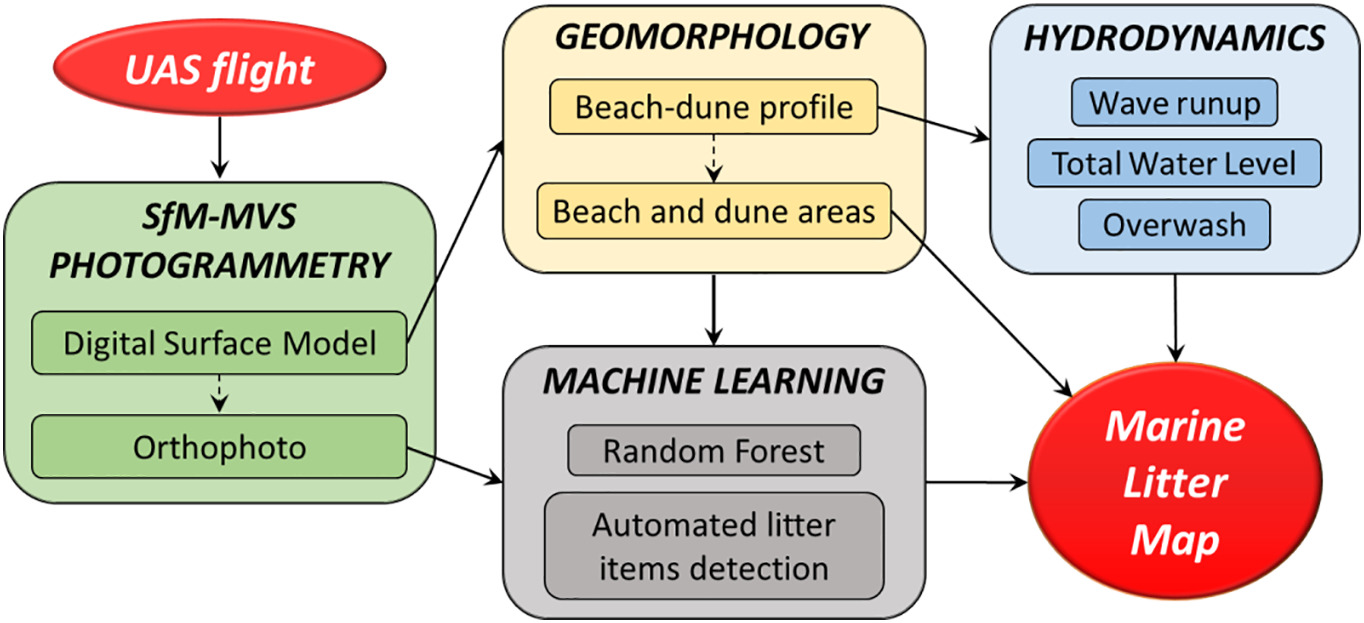
\includegraphics[width=0.6\textwidth,frame]{goncalves2020}
	\caption{A gépi tanulás, geomorfológia, fotogammetria és hidrodinamikai modellezés használása hulladékdetektálásra \cite{Goncalves2020}}
    \label{fig:goncalves2020-method}
\end{figure}

\cite{Youme2021}-ben konvolúciós neuronhálót (CNN) használtak, hogy a Szenegál folyó mentén hulladékot detektáljanak Saint-Louis-ban. A kutatáshoz magas felbontású drónfelvételeket használtak. Drónfelvételeket készítettek 5, 10, 30, illetve 300 méter magasságon, úgy, hogy a látási szög merőleges volt a földre. A 10 méter és 30 méteres felvételeket használták a modell betanítására. A kiválasztott kutatási területnek az az előnye, hogy változatos környezetben található, így modell betanítására és tesztelésére is alkalmas. A modell átlagos pontosságát nem mérték, mivel nagy eltérések voltak a vizsgált régiók függvényében. A cikkben említik, hogy a modell pontossága lényegesen növelhető, ha több adattal kerül betanításra. 

\section{Döntési fa}
\label{ch:decision-tree}

A döntési fák általános célú predikcióra és osztályozásra használt eszközök \cite{deville2013}. Az előnyeik közé tartozik az, hogy tekintve az egyszerű struktúrájukat, könnyen értelmezhetőek és rugalmasak. A \ref{fig:decision-tree} ábrából látható a döntési fa működési elve.

\begin{figure}[H]
	\centering
	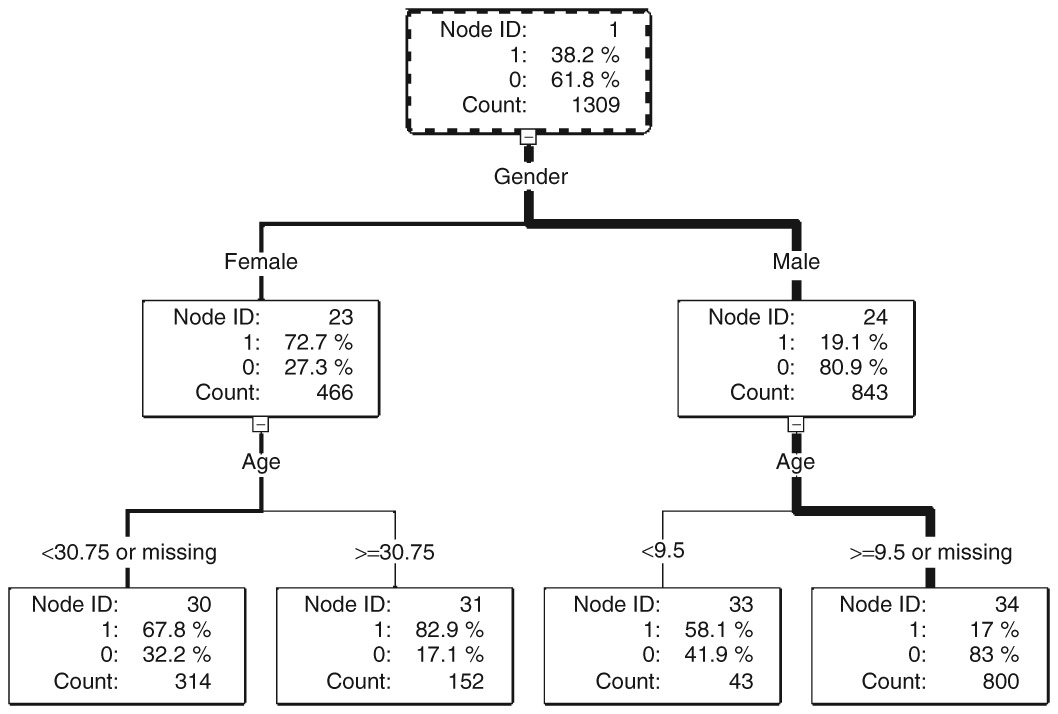
\includegraphics[width=0.6\textwidth,frame]{decision-tree}
	\caption{A döntési fa működési elve \cite{deville2013}}
    \label{fig:decision-tree}
\end{figure}

A \ref{fig:decision-tree} ábrán látható döntési fa a Titanic utasairól készített túlélési kutatás adatai alapján épült \cite{Harrell2013}. A fa csúcsain található 1-es címke képviseli a túlélők arányát, míg a 0-ás címke az elhunytak arányát. Mivel a 0 és 1 osztályok közül választhat a döntési fa, ezért ez egy osztályozó döntési fa. Ezen felül a csúcsban el van tárolva az is, hogy hány mérést tartalmaz. A gyökércsúcs tartalmazza az összes mérést. Ahhoz, hogy leágazzunk egy csúcsból, meg kell határoznunk a közvetlen gyerekcsúcsok "bemeneteit": ezek olyan mezők az adathalmazban, melyek a legjobban leírják a változékonyságát az adatoknak az adott szinten. A legalkalmasabb bemenetek meghatározása egy nyitott kutatási téma. Ebben a példában a gyökércsúcs közvetlen gyerekeinek a bemenete az utas neme. A következő szint bemenete pedig az utas kora. Így például a következő információkat olvashatjuk le a döntési fáról: a 30.75 év fölötti nőknek volt a legnagyobb túlélési esélyük, míg a 9.5 fölötti vagy ismeretlen életkorral rendelkező férfiaknak volt a legkisebb túlélési esélyük. Így tehát ha meg szeretnénk állapítani, hogy mennyi lett volna a túlélési esélye egy 35 éves férfinek, akkor látnánk azt a döntési fa alapján, hogy ez 17\% lenne.

\section{Random Forest}

A \ref{ch:decision-tree} fejezetben tárgyalt döntési fa egyik hátránya az, hogy hajlamos a túltanulásra. A Random Forest egy felügyelt gépi tanulási módszer, mely magas pontossággal tud rátanulni a tanító adatokra (túltanulás nélkül), és jól kezeli a zajt \cite{breiman2001}. A módszer több, véletlenszerűen paraméterezett döntési fa felépítéséből kapta a nevét: miután felépítettük ezt a "döntési fa erdőt", az adatokat úgy lehet osztályozni, hogy egy többségi szavazást hajtunk végre az összes fa eredménye szerint (\ref{fig:random-forest} ábra). Ennek a megközelítésnek köszönhetően az egyes túltanult döntési fák kiegyenlítik egymást, így a teljes erdő nem lesz túltanítva. A fák felépítéséhez több stratégia létezik, és ezen stratégiák alapján lehet finomhangolni a modell pontosságát és méretét. Az utóbbit fontos szem előtt tartani, tekintve arra, hogy elég sok tanító adat esetén a modell mérete lényegesen megnőhet helyes paraméterezés hiányában. Az ilyen paraméterek például a fák maximum mélysége, a fáknak átadott részadathalmaz dimenziói, egy csúcs kettéválasztásának a kritériumjai, a tanító adatok súlyai stb. A kutatásomban ezt a modellt tanítom be, illetve paraméterezem azzal a céllal, hogy megbízható klasszifikációt tudjon biztosítani. A modell minden képkockát osztályozni fog, így a bemeneti adatok az adott terület spektrális sávjai, illetve indexei. 

\begin{figure}[H]
	\centering
	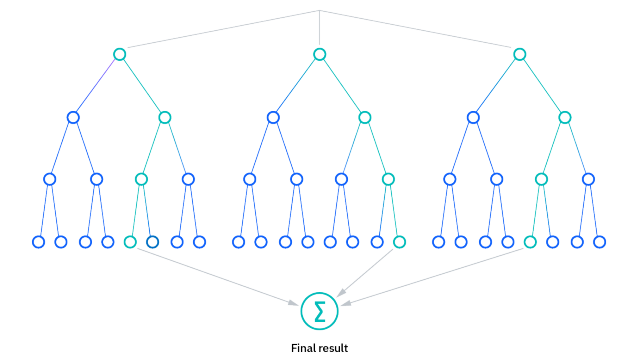
\includegraphics[width=0.5\textwidth,frame]{random-forest}
	\caption{A Random Forest működési elve \cite{IBM2024}}
    \label{fig:random-forest}
\end{figure}

\section{PlanetScope}

A Planet Labs rendszeresen műholdakat küld az űrbe azzal a céllal, hogy minden nap készüljön műholdfelvétel a Földről \cite{planetgoal2024}. A projekt jelenlegi állapotában már ott tartanak, hogy majdnem napi szintű felvételeket készítenek a Föld felszínéről több, mint 430 Dove és SuperDove műhold segítségével \cite{planetmissions2024}. A legújabb műholdcsaládjuk a SuperDove műholdakból áll. Ezek a műholdak a PSB.SD nevű műszert használják felvételek készítésére. A műszer a 47 megapixeles "PSBlue" szenzort használja.  Ezekkel a műholdakkal 2020. március közepe óta készítenek felvételeket, melyek a vörös (red), zöld (green), kék (blue), közeli infravörös (near infrared vagy NIR), illetve az úgynevezett "red edge", "green I", "coastal blue", és sárga (yellow) sávokat is tartalmazzák. Egy csempe körülbelül 32.5 x 19.6 $ km^2 $ területet fed le \cite{planetsensors2024}, körülbelül 3 méter per pixel felbontással. A \ref{tab:planet-wavelengths} táblázatból látható, hogy a PSB.SD műszer egyes sávjai milyen hullámhosszal rendelkeznek. A hullámhossz mellett jelenített "fwhm" a "Full width at half maximum" értéknek a rövidítése.

\begin{table}[H]
	\centering
	\begin{tabular}{ | p{0.2\textwidth} | p{0.2\textwidth} | p{0.2\textwidth} | }
		\hline
		\textbf{Sáv azonosító} & \textbf{Sáv neve} & \textbf{Hullámhossz (fwhm)} \\
		\hline \hline
		1 & Coastal Blue & 443 (20) \\
		\hline
		2 & Blue & 490 (50) \\
		\hline
		3 & Green I & 531 (36) \\
		\hline
        4 & Green & 565 (36) \\
		\hline
		5 & Yellow & 610 (20) \\
		\hline
		6 & Red & 665 (31) \\
		\hline
		7 & Red Edge & 705 (15) \\
		\hline
        8 & NIR & 865 (40) \\
		\hline
	\end{tabular}
	\caption{A PSB.SD műszer hullámhosszai \cite{planetsensors2024}}
	\label{tab:planet-wavelengths}
\end{table}

